\section{Laboratorio de Active Directory}

En la siguiente sección se van a establecer las directrices para la creación de un laboratorio local que permita la realización de los ataques que se describirán y ex\-pe\-ri\-men\-ta\-rán en los capítulos previos a este. La organización de este capítulo es la siguiente: en primer lugar se detallan los requisitos o prerrequisitos necesarios para poder realizar las siguientes acciones como puede ser el software de virtualización, las imágenes del sistema operativo, etc. Posteriormente, se ha definido y configurado la topología elegida y por último la instalación y administración de Active Directory. 

\subsection{Requisitos}

Previamente a la creación de la topología de red y a la instalción de Active Directory que permita realizar las pruebas es necesario disponer de las siguientes características.

\subsubsection{Software de virtualización}

La virtualización consiste en la creación de entornos simulados o recursos desde un único sistema operativo denominado {\it host}, por consecuencia, un software de virtualización es aquel que te permite realizar las acciones descritas anteriormente que puede ser la creación de sistemas operativos, creación de topologías de red, administración de recursos, etc. Aunque hay gran variedad de software de virtualización, para la realización de este proyecto se ha utilizado {\it Oracle VM VirtualBox}~\cite{Capitulo4:VirtualBox}.\\

{\it VirtualBox} es un software de virtualización {\it Open Source} con licencia GPLv2 desarrollado por Oracle Corporation que permite la creación de entornos x86 and AMD64/Intel64. Para este proyecto se ha utilizado la última versión (VirtualBox 6.0.12) que se puede descargar en \footnote{https://www.virtualbox.org/}. Con este software se van a crear las máquinas virtuales y las redes internas necesarias para la creación del laboratorio. 

\subsubsection{Máquinas Virtuales}

Para este proyecto se van a utilizar cuatro máquinas virtuales. Para aquellas que se necesite una licencia de software privativo se va a utilizar la versión de prueba que proporciona Microsoft con el objetivo de que cualquiera pueda replicar dicho laboratorio sin necesidad de lincencias adicionales. Las máquinas son las siguientes:

\begin{itemize}
\item \textbf{DC01}: Es la máquina virtual principal y es la encargada de administrar el Active Directory. Como se ha comentado en el estado del arte se va a utilizar Windows Server 2019 es su última versión. La imagen del sistema operativo se ha descargado de \footnote{https://www.microsoft.com/en-us/evalcenter/evaluate-windows-server-2019}.

\item \textbf{Cliente01}: Por otro lado, esta máquina representa a la de un usuario legítimo o cliente de una empresa que está unido al dominio y conectado por la red interna. Para esta máquina virtual se ha utilizado Windows 10 Enterprise que se puede descargar en \footnote{https://www.microsoft.com/en-us/evalcenter/evaluate-windows-server-2019}. 

\item \textbf{Gateway}: Esta máquina virtual se va a utilizar como puerta de enlace entre la red interna y la red externa lo que simula ser internet. Para su implementación, se ha utilizado Debian 10 (Buster) sin escritorio para ahorrar recursos locales. La imagen de este sistema operativo se puede descargar en \footnote{https://cdimage.debian.org/debian-cd/current/amd64/iso-cd/debian-10.1.0-amd64-netinst.iso}.

\item \textbf{Atacante01}: Por último, para la simulación de un atacante externo o profesional de la seguridad ofensiva realizando labores de {\it Red Team}, se ha utilizado la distribución Kali Linux 2019.3. Esta distribución ofrece gran variedad de herramientas destinadas a la auditoría informática que serán de utilidad a la hora de realizar los ataques propuestos. Para descargar esta distribución se puede a través de \footnote{https://cdimage.kali.org/kali-2019.3/kali-linux-2019.3-amd64.iso}.

\end{itemize}


\subsubsection{Instalación y actualización}

La instalación y actualización de las máquinas, no se ha considerado como alcance de este proyecto, por lo tanto, a partir de este punto se da por hecho que el usuario ha instalado y actualizado las máquinas y cuenta con la última versión de las mismas. 

\subsection{Configuración previa}

Antes de configurar el Active Directory, se ha creado una topología en red que simula a un entorno coorporativo fictio. Aunque este laboratorio únicamente disponga de una máquina unida al dominio, en entornos reales son multitud los equipos unidos al dominio, lo que posibilita un gran abanico de posibles entradas a la red de la empresa u organización. A continuación se va a explicar la topología elegida y las configuraciones necesarias.

\subsubsection{Topología de red}

Como ya se ha adelantado, la máquina consta de 4 máquinas: 2 Windows (DC01 y Cliente01) y 2 Linux (Atacante01 y Gateway). La distribución de la topología en red se puede observar en la Figura \ref{Topología}. En la imagen se puede apreciar la existencia de dos redes: ADNET(192.168.0.0/24) formada por los dos dos Sistemas Windows que forman parte del dominio de la empresa fictia y EXTNET(10.10.10.0) que emula en una red interna lo que sería estar expuesto a internet en un entorno real. Ambas redes están enlazadas por el Gateway. 

\begin{figure}[H] %[ht!] para here [b] para bottom [t] para top
\begin{center}
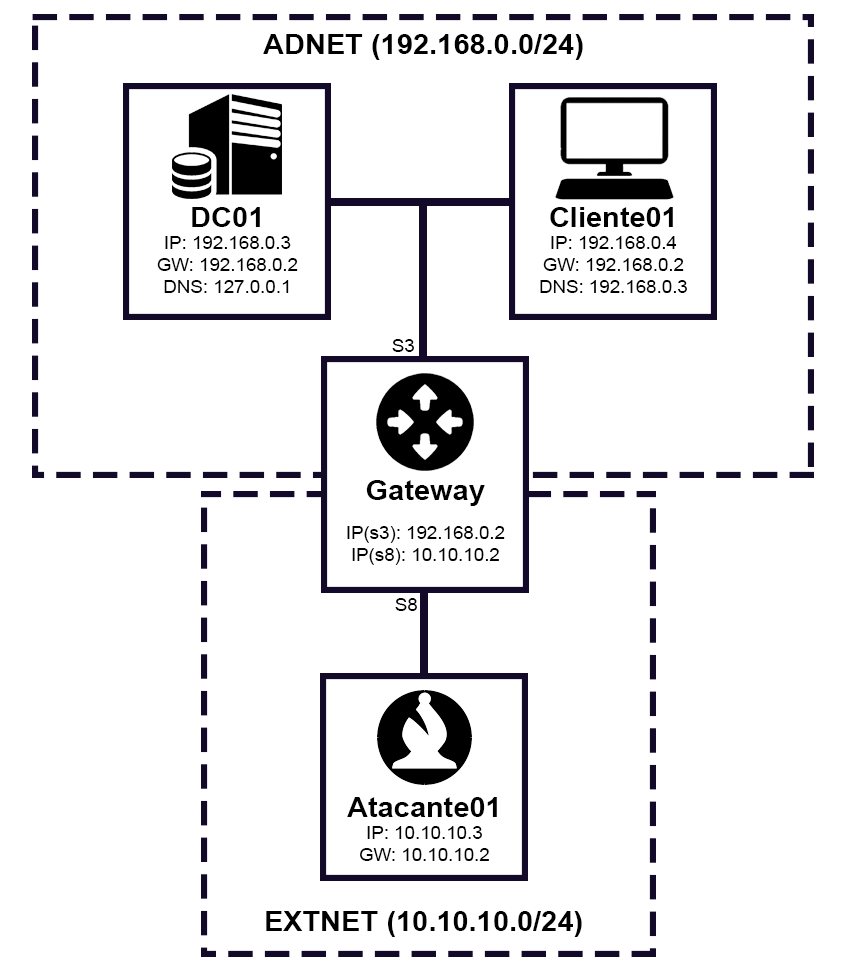
\includegraphics[width=16cm]{Topologia.png}
\end{center}
\caption{Topología del laboratorio local.}
\label{Topología}
\end{figure}

\subsubsection{Configuración de red}

Se va a realizar la configuración necesaria para cada red. 

\begin{itemize}
\item \textbf{DC01}
\begin{enumerate}
\item Antes de arrancar la máquina virtual, es necesario ir a Configuración/Red y añadir el Adaptador1. Esto va a simular la tarjeta de red del DC01. Esta tarjeta de red la vamos a conectar a la red ADNET como se puede ver en la Figura \ref{DC01-Red1}.

\begin{figure}[H] %[ht!] para here [b] para bottom [t] para top
\begin{center}
\includegraphics[width=16cm]{DC01/Red1.png}
\end{center}
\caption{Configuración de red DC01 - Tarjeta de red.}
\label{DC01-Red1}
\end{figure}

\item Una vez iniciada la máquina es necesario dirigirse a {\it Control Panel - Network and Internet - Network Connections} (Figura \ref{DC01-Red2}) y aparecerá la tarjeta de red añadida en el paso anterior. Para editar las direcciones es necesario entrar a las propiedades.
\begin{figure}[H] %[ht!] para here [b] para bottom [t] para top
\begin{center}
\includegraphics[width=16cm]{DC01/Red2.png}
\end{center}
\caption{Configuración de red DC01 - Ajustes de Ethernet.}
\label{DC01-Red2}
\end{figure}

\item Por último, como se puede observar en la Figura \ref{DC01-Red3}, se elige {\it Internet Version Protocol 4(TCP/IPv4) } y después las propiedades de este. Por último, se configura la dirección IP (192.168.0.3), la puerta de enlace correspondiente al Gateway (192.168.0.2) y el DNS. En la mayoría de entornos corporativos es el propio Active Directory el que hace la función de servidor DNS, por lo tanto se escribe la dirección de {\it loopback}: 127.0.0.1.
\begin{figure}[H] %[ht!] para here [b] para bottom [t] para top
\begin{center}
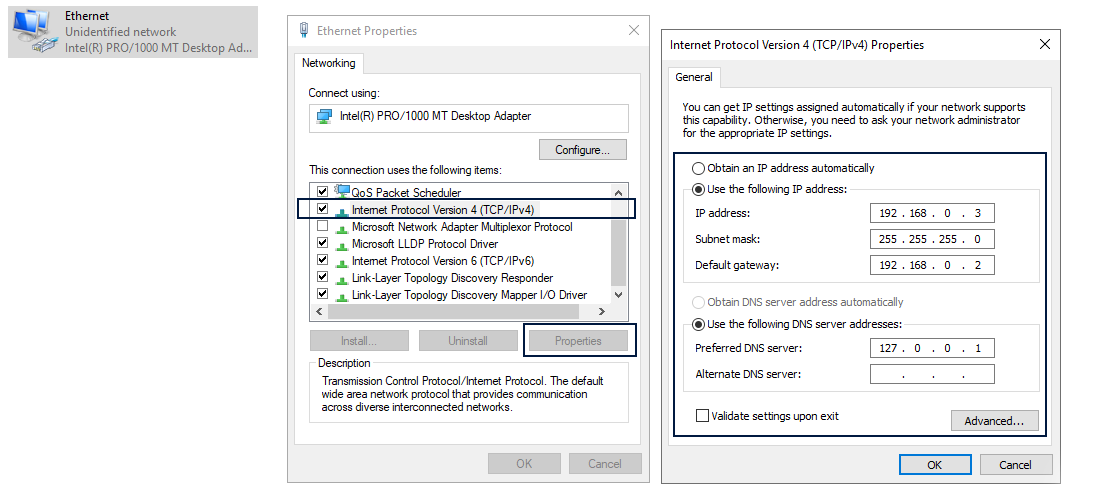
\includegraphics[width=16cm]{DC01/Red3.png}
\end{center}
\caption{Configuración de red DC01 - IPv4.}
\label{DC01-Red3}
\end{figure}
\end{enumerate}

\item \textbf{Cliente01}:
\begin{enumerate}
\item Para configurar la red en el Cliente01, al ser una máquina Windows en la misma red que el DC01, es necesario repetir los mismos pasos que en la configuración anterior.
\item En el último paso, las direcciones IP son las siguientes: IP(192.168.0.4) y Gateway(192.168.0.2). En este caso la dirección DNS corresponde a la di\-re\-cción IP del DC01: 192.168.0.3. La configuración resultante se puede ver en la Figura \ref{Cliente01-Red1}.

\begin{figure}[H] %[ht!] para here [b] para bottom [t] para top
\begin{center}
\includegraphics[width=10cm]{Cliente01/Red1.png}
\end{center}
\caption{Configuración de red Cliente01 - IPv4.}
\label{Cliente01-Red1}
\end{figure}
\end{enumerate}

\item \textbf{Gateway}:

\begin{enumerate}
\item Para esta máquina, es necesario habilitar dos interfaces, una que corresponde a la ADNET o red interna y otra que corresponde con la EXTNET o red externa (Figura \ref{Gateway-Red1}).
\begin{figure}[H] %[ht!] para here [b] para bottom [t] para top
\begin{center}
\includegraphics[width=10cm]{Gateway/Red1.png}
\end{center}
\caption{Configuración de red Gateway - Tarjetas de red.}
\label{Gateway-Red1}
\end{figure}

\item Iniciamos la máquina y comprobamos que se han creado ambas interfaces {\it enp0s3} para la ADNET y {\it enp0s8} para la EXTNET. 

\item A continuación introducimos los siguientes comandos. Estos comandos levantan ambas interfaces y asignan las direcciones IP correspondientes. 
\begin{listing}[style=consola, numbers=none]
# ip link set enp0s3 up
# ip a add 192.168.0.2/24 dev enp0s3
# ip link set enp0s8 up
# ip a add 10.10.10.2/24 dev enp0s8
\end{listing}

\item Por último, permitimos que el gateway reenvíe los paquetes que le llegan. Para eso se utiliza el siguiente comando: 
\begin{listing}[style=consola, numbers=none]
# echo 1 > /proc/sys/net/ipv4/ip_forward
\end{listing}

\item La configuración final de la máquina se puede observar en la Figura \ref{Gateway-Red2}.
\begin{figure}[H] %[ht!] para here [b] para bottom [t] para top
\begin{center}
\includegraphics[width=15cm]{Gateway/Red2.png}
\end{center}
\caption{Configuración de red Gateway}
\label{Gateway-Red2}
\end{figure}
\end{enumerate}

\item \textbf{Atacante01}:

\begin{enumerate}

\item Esta máquina está en la red externa, por lo tanto añadimos un adaptador de red unida a la red externa (Figura \ref{Atacante01-Red1}). 
\begin{figure}[H] %[ht!] para here [b] para bottom [t] para top
\begin{center}
\includegraphics[width=10cm]{Atacante01/Red1.png}
\end{center}
\caption{Configuración de red Atacante01 - Tarjeta de red}
\label{Atacante01-Red1}
\end{figure}

\item De la misma manera que en el gateway, configuramos la interfaz de red, que en este caso es {\it eth0} con los siguientes comandos. 
\begin{listing}[style=consola, numbers=none]
# ip link set eth0 up
# ip a add 10.10.10.3 dev eth0 
\end{listing}

\item Para poder alcazar la red interna, es necesario definir a la dirección 10.10.10.2 como gateway, para que cuando la máquina no encuentre una dirección IP la redirija por ese Gateway. Para ello, se utiliza el siguiente comando: 

\begin{listing}[style=consola, numbers=none]
# ip route default via 10.10.10.2
\end{listing}

\end{enumerate}
\end{itemize}

\subsubsection{Comprobación de la conectividad}

\begin{itemize}

\item \textbf{Cliente01 - DC01}: Para comprobar la conectividad entre Cliente01 y DC10, podemos realizar un ping desde Cliente01 a la dirección IP de DC01 (\ref{Cliente01-Red2}).
\begin{figure}[H] %[ht!] para here [b] para bottom [t] para top
\begin{center}
\includegraphics[width=10cm]{Cliente01/Red2.png}
\end{center}
\caption{Conexión entre Cliente01 y DC01}
\label{Cliente01-Red2}
\end{figure}

\item \textbf{Atacante01 - DC01}: Para comprobar la conectividad entre Atacante01 y DC10, en vez de realizar un ping intentamos conectarnos a través de Samba (\ref{Atacante01-Red2})
\begin{figure}[H] %[ht!] para here [b] para bottom [t] para top
\begin{center}
\includegraphics[width=10cm]{Atacante01/Red2.png}
\end{center}
\caption{Conexión entre Atacante01 y DC01}
\label{Atacante01-Red2}
\end{figure}

\end{itemize}

\subsubsection{Cambio de nombre del sistema}

Una buena práctica es cambiar el nombre a los Sistemas Windows, esto nos facilitará su identificación y su futura administración. 

\begin{itemize}
\item Para cambiar el nombre a DC01, se puede realizar desde el propio panel de ad\-mi\-nis\-tra\-ción del servidor, a través de la opción {\it Local Name Server - Computer Name - Change} como se puede ver en la Figura \ref{DC01-Name1}
\begin{figure}[H] %[ht!] para here [b] para bottom [t] para top
\begin{center}
\includegraphics[width=15cm]{DC01/Name1.png}
\end{center}
\caption{Cambio de nombre DC01}
\label{DC01-Name1}
\end{figure}

\item Para cambiar el nombre a Cliente01, se realiza a través de {\it Control Panel - System and Security - System}. Posteriormente, se elige la opción {\it Change Settings - Change} y se introduce el nombre Cliente01 (\ref{Cliente01-Name1}). Ambos cambios nos van a pedir un reinicio del equipo. 
\begin{figure}[H] %[ht!] para here [b] para bottom [t] para top
\begin{center}
\includegraphics[width=13cm]{Cliente01/Name1.png}
\end{center}
\caption{Cambio de nombre Cliente01}
\label{Cliente01-Name1}
\end{figure}

\end{itemize}

\subsection{Creación y configuración del Active Directory}

En esta sección se va a detallar la instalación y configuración de Active Directory en Windows Server 2019 en la máquina virtual DC01.

\subsubsection{Intalación y configuración}

\begin{enumerate}

\item La instalación de un AD DS se puede realizar desde el Dashboard integrado en Windows Server 2019. Para ello, se selecciona {\it Add roles and features} (Figura \ref{DC01-AD1}).
\begin{figure}[H] %[ht!] para here [b] para bottom [t] para top
\begin{center}
\includegraphics[width=15cm]{DC01/AD1.png}
\end{center}
\caption{Instalación de AD DS - Add roles and features.}
\label{DC01-AD1}
\end{figure}


\item Para el tipo de instalación se va a elegir {\it Role-based or feature-based installation} (Figura \ref{DC01-AD2}).
\begin{figure}[H] %[ht!] para here [b] para bottom [t] para top
\begin{center}
\includegraphics[width=15cm]{DC01/AD2.png}
\end{center}
\caption{Instalación de AD DS - Role-based installation.}
\label{DC01-AD2}
\end{figure}


\item Después elegimos el DC01 (o el nombre que se haya elegido al cambiar el nombre en la sección anterior) como se puede ver en la Figura \ref{DC01-AD3}.
\begin{figure}[H] %[ht!] para here [b] para bottom [t] para top
\begin{center}
\includegraphics[width=15cm]{DC01/AD3.png}
\end{center}
\caption{Instalación de AD DS - DC01.}
\label{DC01-AD3}
\end{figure}


\item En la sección {\it Server Roles} se elige Active Directory Domain Services (Figura \ref{DC01-AD4}), al seleccionar esta opción se desplegará un menú donde debemos especifiar las caracterísitcas, se seleciona en {\it Add Features}.
\begin{figure}[H] %[ht!] para here [b] para bottom [t] para top
\begin{center}
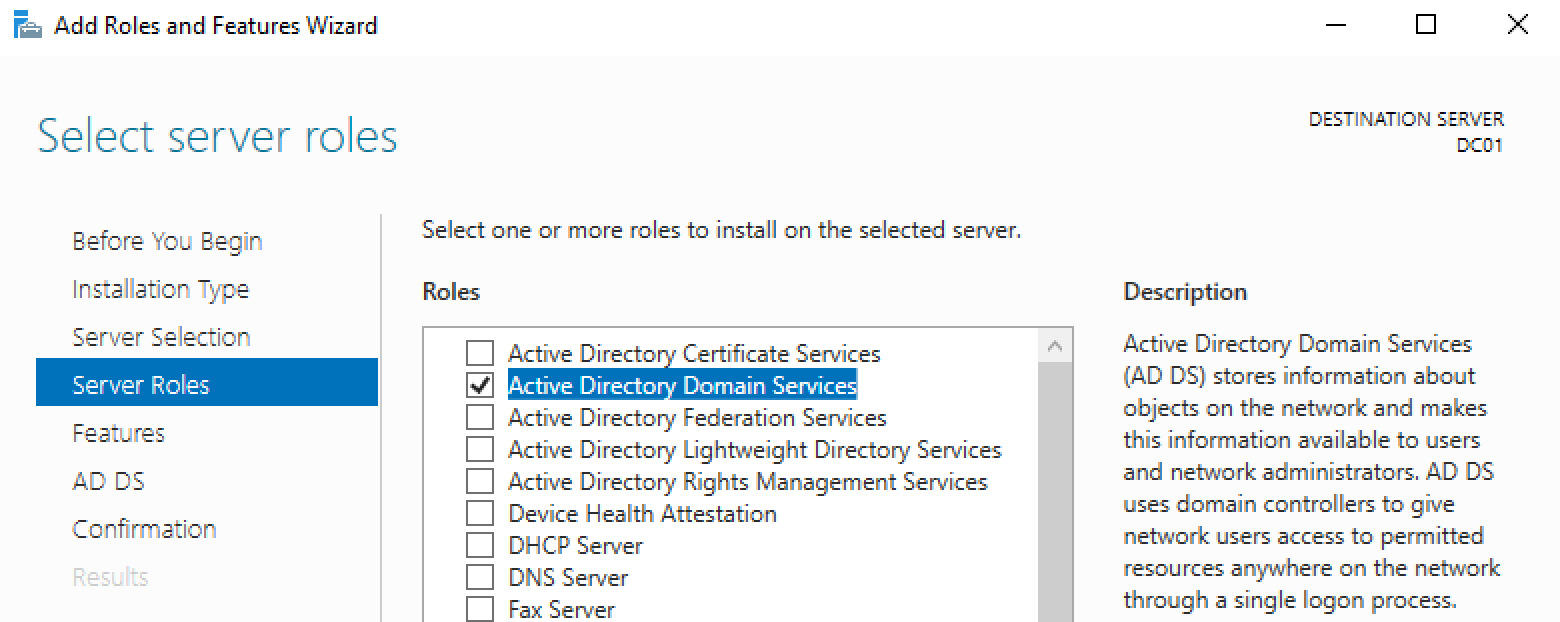
\includegraphics[width=15cm]{DC01/AD4.png}
\end{center}
\caption{Instalación de AD DS - Active Directory Domain Services.}
\label{DC01-AD4}
\end{figure}


\item Después seguimos la instalción hasta la opción {\it Confirmation} e instalamos AD DS (Figura \ref{DC01-AD5}).
\begin{figure}[H] %[ht!] para here [b] para bottom [t] para top
\begin{center}
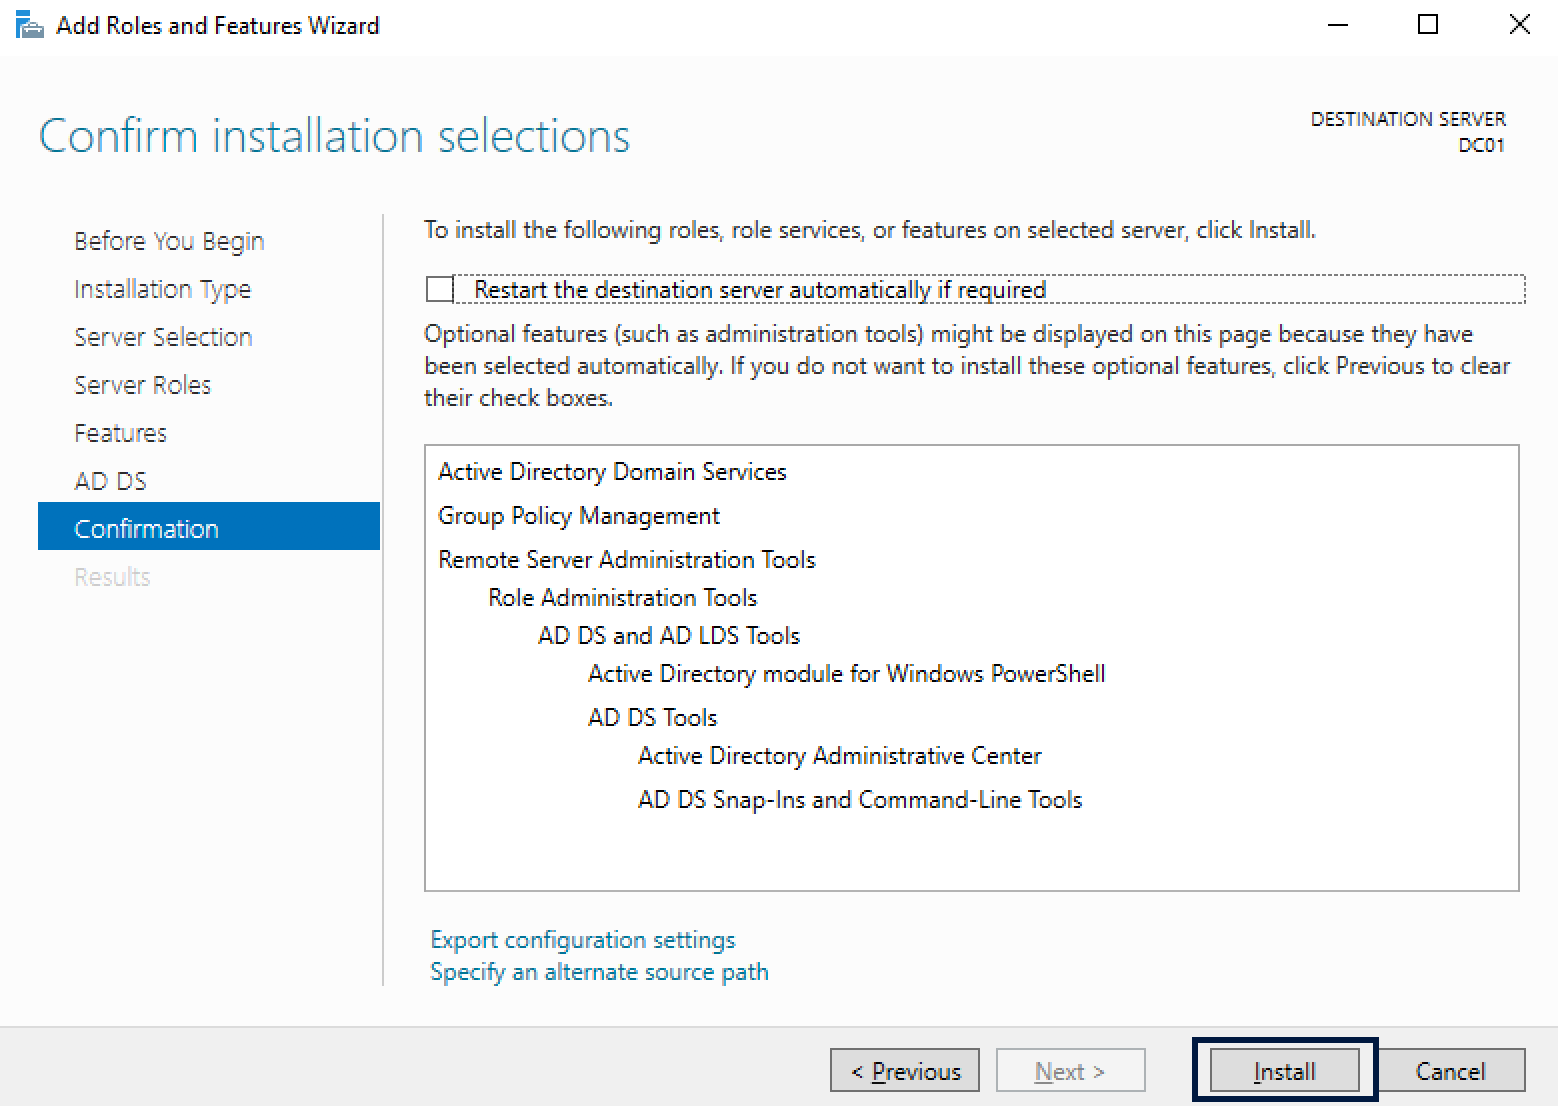
\includegraphics[width=15cm]{DC01/AD5.png}
\end{center}
\caption{Instalación de AD DS - Instalación.}
\label{DC01-AD5}
\end{figure}


\item Cuando se termina la instalación se debe ``promocionar'' el servidor DC01 como Domain Controller, para ello seleccionamos la opción que se puede ver en la Figura \ref{DC01-AD6}.
\begin{figure}[H] %[ht!] para here [b] para bottom [t] para top
\begin{center}
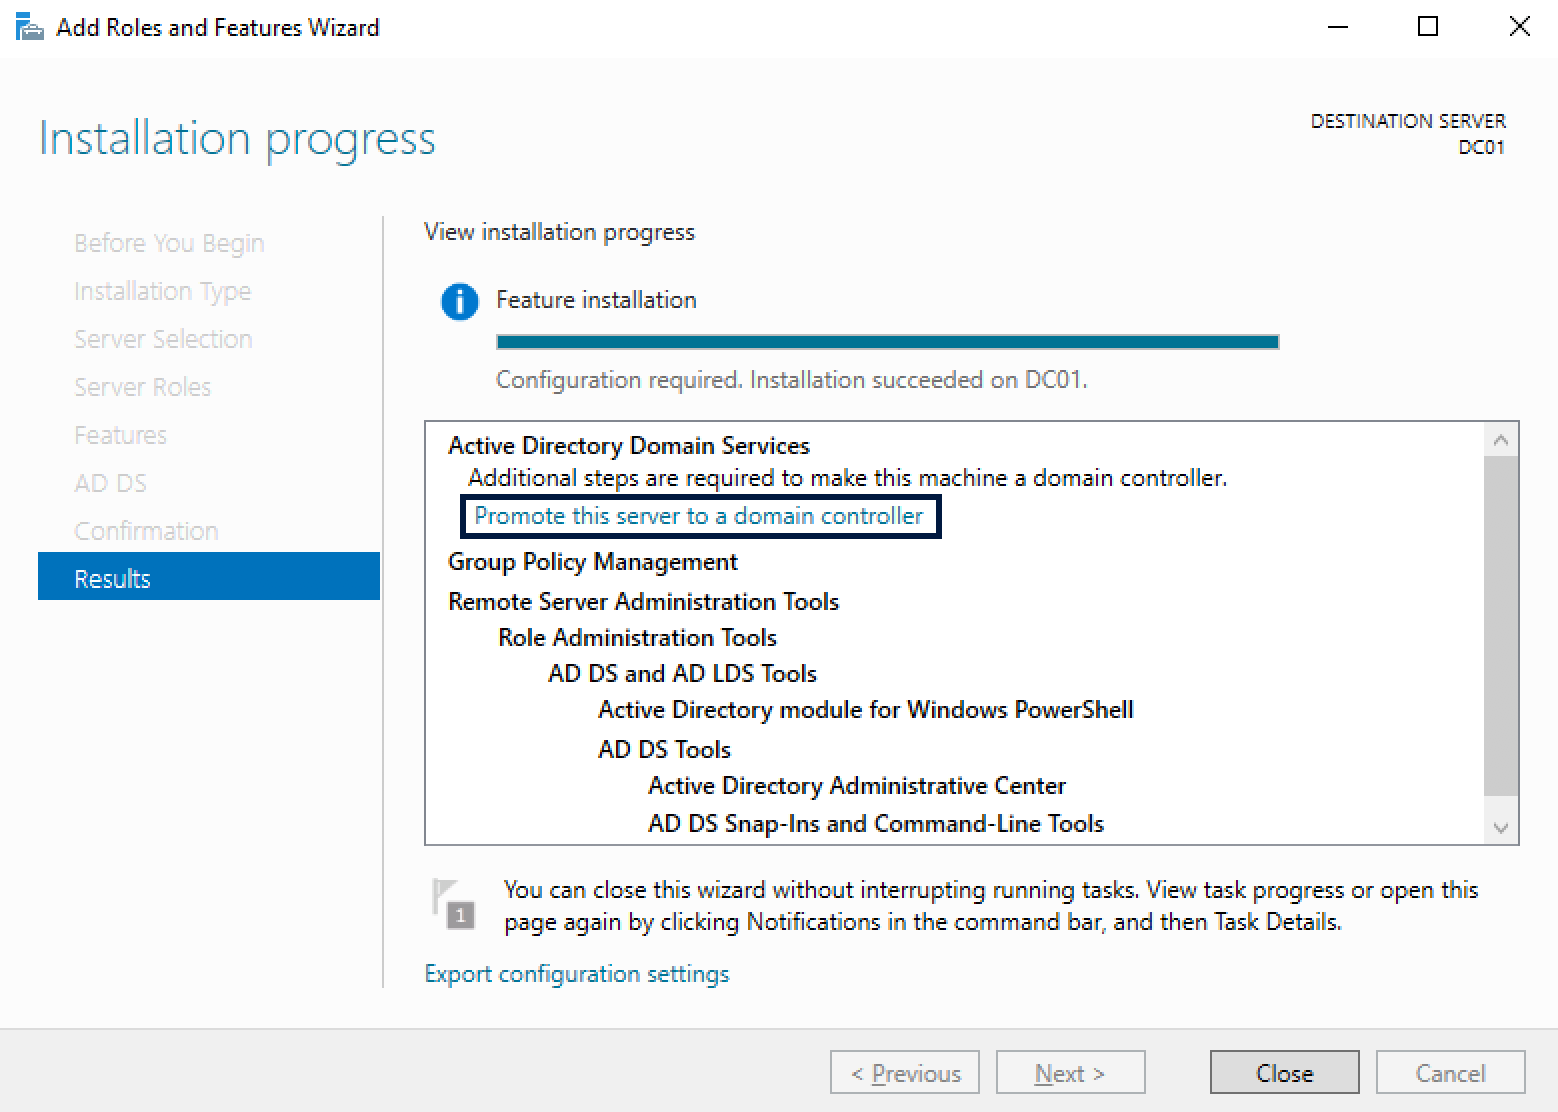
\includegraphics[width=15cm]{DC01/AD6.png}
\end{center}
\caption{Instalación de AD DS - Promote to Domain Controller.}
\label{DC01-AD6}
\end{figure}


\item Posteriormente, al no disponer de ningún forest previo, es necesario crear uno con el nombre {\it laboratory.com} (Figura \ref{DC01-AD7}). 
\begin{figure}[H] %[ht!] para here [b] para bottom [t] para top
\begin{center}
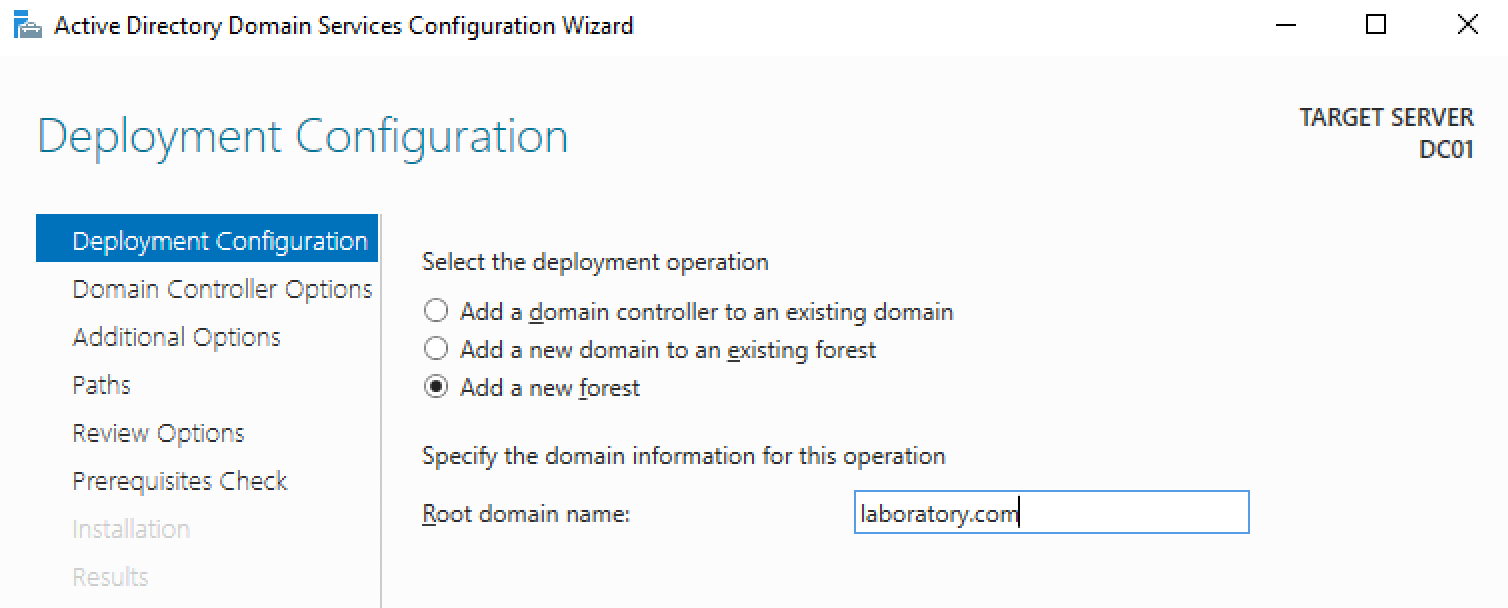
\includegraphics[width=15cm]{DC01/AD7.png}
\end{center}
\caption{Instalación de AD DS - Creación del forest laboratory.com.}
\label{DC01-AD7}
\end{figure}


\item En la pestaña {\it Domain Controller Options} elegimos Windows Server 2016 al ser la versión más actualizada posible, después si no se dispone de un DNS externo, se elige que el Domain Controller tenga la capacidad de DNS y Global Catalog. Además, se elige la contraseña para el Directory Services Restore Mode (DSRM) (Figura \ref{DC01-AD8}).
\begin{figure}[H] %[ht!] para here [b] para bottom [t] para top
\begin{center}
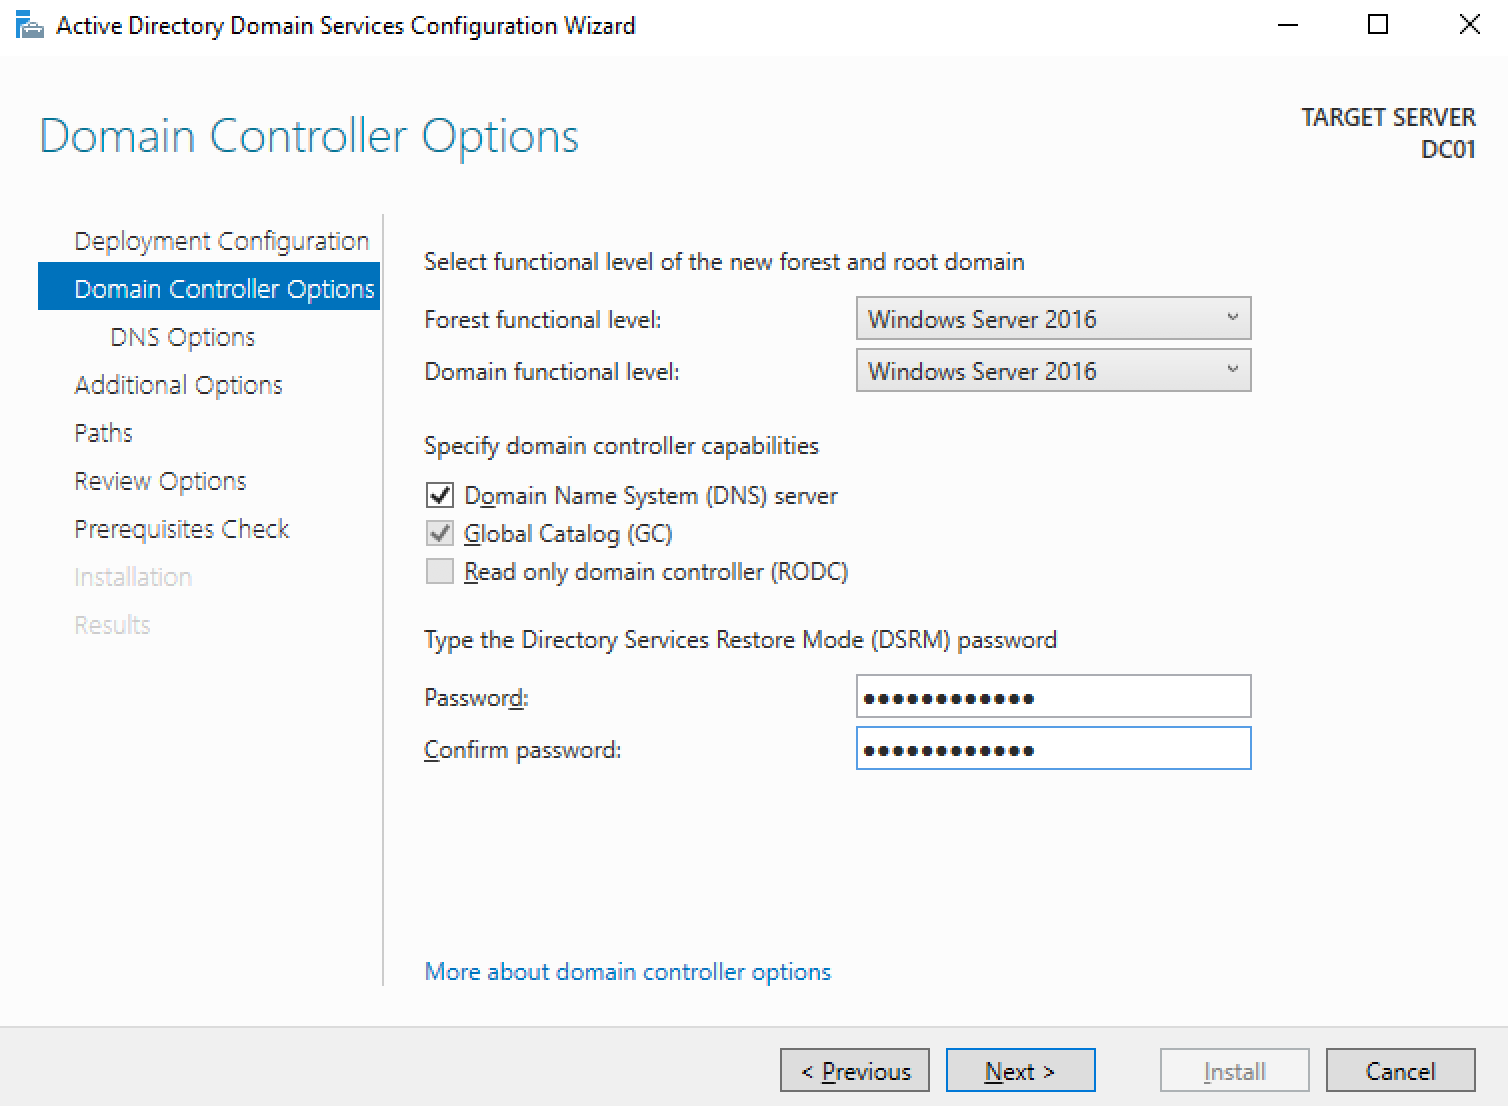
\includegraphics[width=15cm]{DC01/AD8.png}
\end{center}
\caption{Instalación de AD DS - Domain Controller options.}
\label{DC01-AD8}
\end{figure}


\item En la pestaña de {\it Paths} podemos ver las rutas de los principales elementos del DC como puede ser la base de datos NTDS y la carpeta SYSVOL (Figura \ref{DC01-AD9}).
\begin{figure}[H] %[ht!] para here [b] para bottom [t] para top
\begin{center}
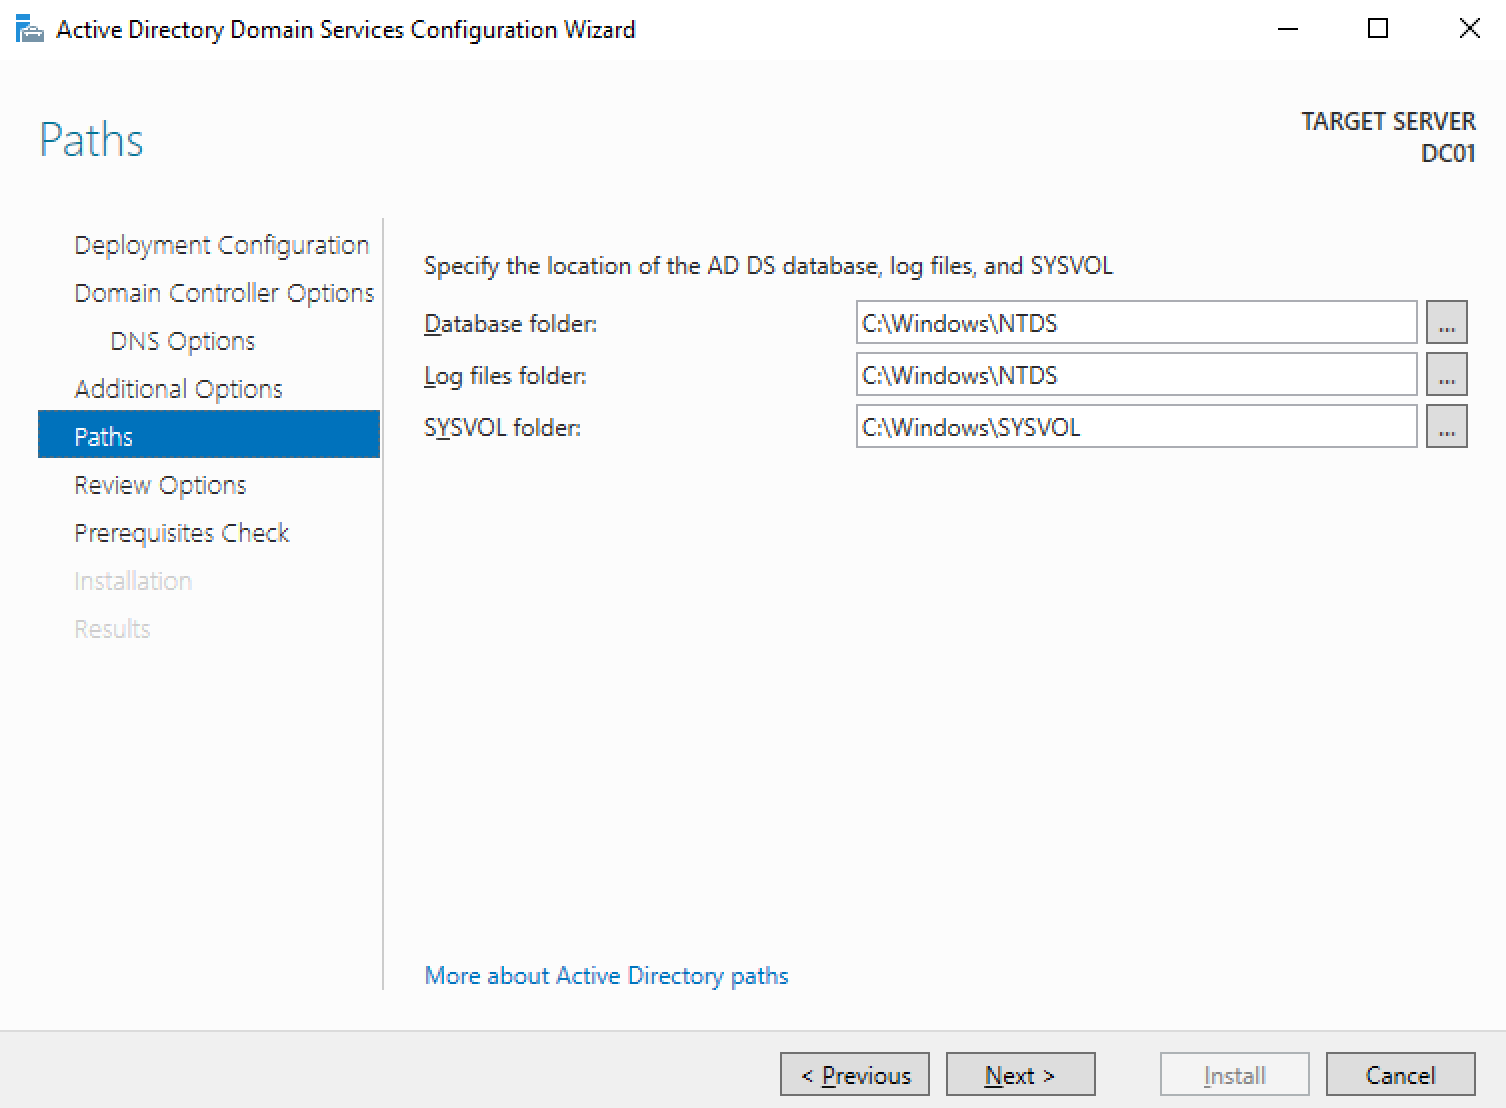
\includegraphics[width=15cm]{DC01/AD9.png}
\end{center}
\caption{Instalación de AD DS - Rutas NTDS y SYSBOL.}
\label{DC01-AD9}
\end{figure}

\item Por último, instalamos las opciones definidas anteriormente Figura \ref{DC01-AD10}. Después de esta opción es necesario reiniciar el servidor. 
\begin{figure}[H] %[ht!] para here [b] para bottom [t] para top
\begin{center}
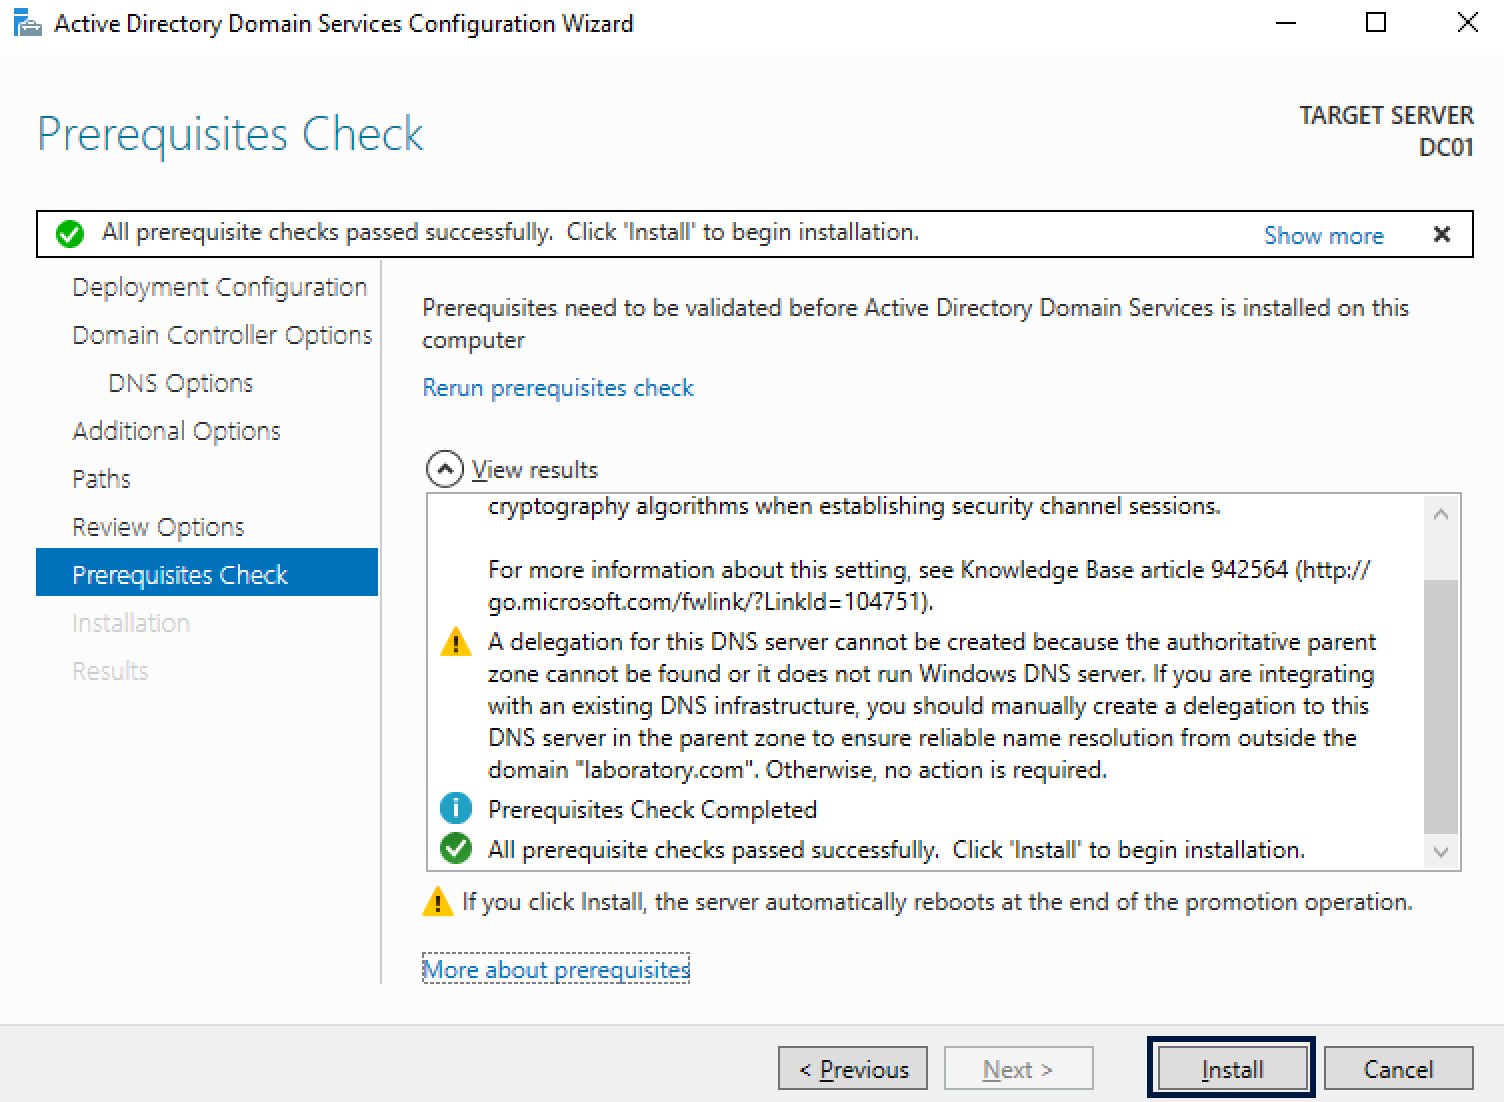
\includegraphics[width=15cm]{DC01/AD10.png}
\end{center}
\caption{Instalación de AD DS - Instalación.}
\label{DC01-AD10}
\end{figure}

\end{enumerate}

\subsubsection{Enlazar cliente al dominio}

Para añadir Cliente01 al dominio {\it laboratory.com} es necesario realizar los siguientes pasos: 

\begin{enumerate}
\item Del mismo modo que para cambiar el nombre al equipo, es necesario ir a {\it Control Panel - System and Security - System}, después realizar click en {\it Change settings} (Figura \ref{Cliente01-AD1}). 
\begin{figure}[H] %[ht!] para here [b] para bottom [t] para top
\begin{center}
\includegraphics[width=15cm]{Cliente01/AD1.png}
\end{center}
\caption{Enlazar cliente al dominio - Settings.}
\label{Cliente01-AD1}
\end{figure}

\item Después se selecciona {\it change} y en la opción de {\it Member of - Domain} se elige el dominio {\it laboratory.com} (Figura \ref{Cliente01-AD2}).
\begin{figure}[H] %[ht!] para here [b] para bottom [t] para top
\begin{center}
\includegraphics[width=15cm]{Cliente01/AD2.png}
\end{center}
\caption{Enlazar cliente al dominio - Dominio.}
\label{Cliente01-AD2}
\end{figure}


\item Al confirmar este cambio se requiere las credenciales del Domain Admin (Figura \ref{Cliente01-AD3}) y reiniciar el sistema.
\begin{figure}[H] %[ht!] para here [b] para bottom [t] para top
\begin{center}
\includegraphics[width=10cm]{Cliente01/AD3.png}
\end{center}
\caption{Enlazar cliente al dominio - Log on.}
\label{Cliente01-AD3}
\end{figure}

\item Finalmente, se puede confirmar que la operación se ha realizado correctamente desde el DC01 desde la opción {\it Tools - Active Directory Users and Computers - Laboratory.com - Computers} (Figura \ref{DC01-AD12}) del Dashboard como se puede ver en la Figura \ref{DC01-AD11}. 
\begin{figure}[H] %[ht!] para here [b] para bottom [t] para top
\begin{center}
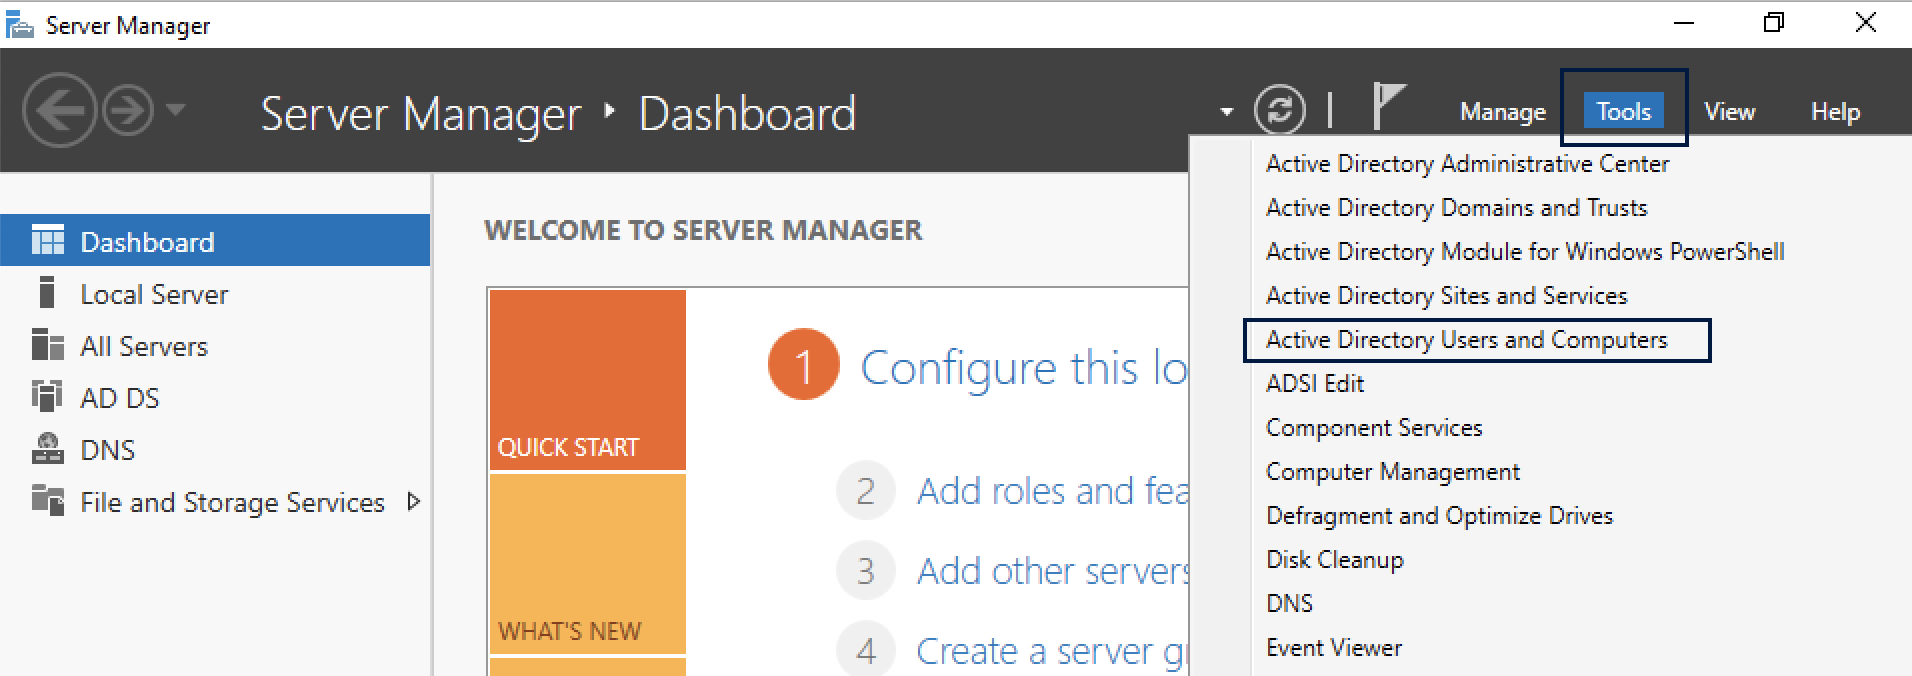
\includegraphics[width=15cm]{DC01/AD12.png}
\end{center}
\caption{Enlazar cliente al dominio - Users and Computers.}
\label{DC01-AD12}
\end{figure}

\begin{figure}[H] %[ht!] para here [b] para bottom [t] para top
\begin{center}
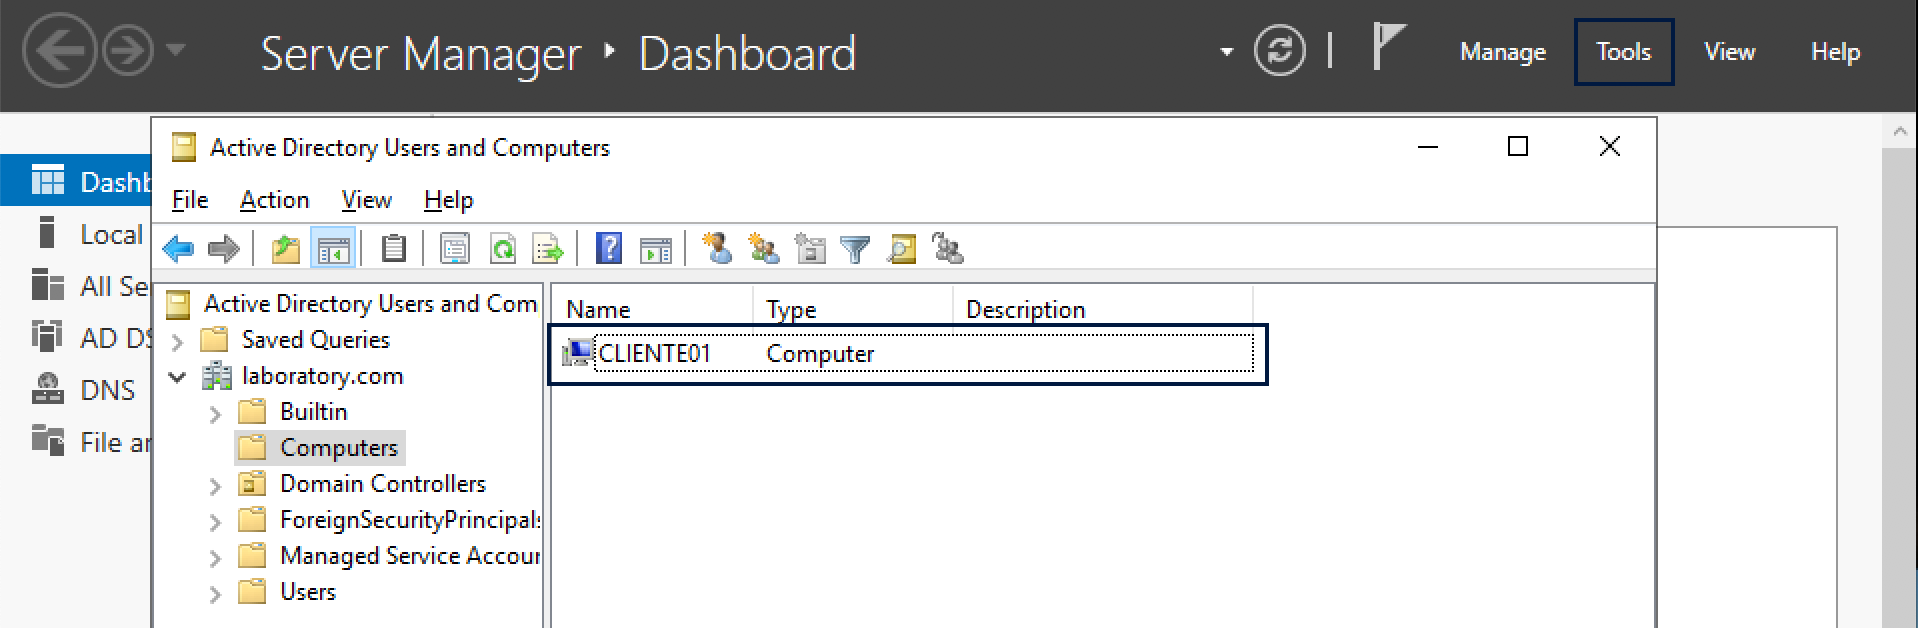
\includegraphics[width=15cm]{DC01/AD11.png}
\end{center}
\caption{Enlazar cliente al dominio - Dashboard.}
\label{DC01-AD11}
\end{figure}


\end{enumerate}

\subsubsection{Creación de usuarios}

Para la fase de experimentación, además, se van a crear tres usuarios con distintos privilegios de administración en el dominio. Para ello, desde DC01 se elige la opción {\it Tools - Active Directory Users and Computers - Laboratory.com - Computers} (Figura \ref{DC01-AD12}) y después se selecciona {\it Users - New - User} como en la Figura \ref{DC01-AD13}. 

\begin{figure}[H] %[ht!] para here [b] para bottom [t] para top
\begin{center}
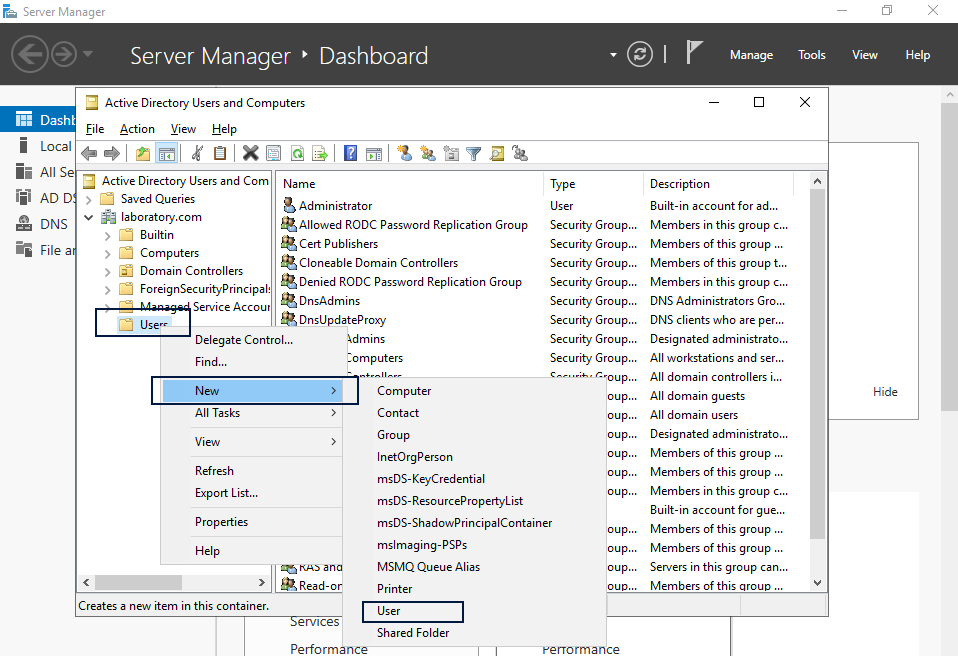
\includegraphics[width=15cm]{DC01/AD13.png}
\end{center}
\caption{Crear nuevo usuario.}
\label{DC01-AD13}
\end{figure}

\begin{itemize}

\item Usuario de dominio (Figura \ref{DC01-User1}). 
\begin{figure}[H] %[ht!] para here [b] para bottom [t] para top
\begin{center}
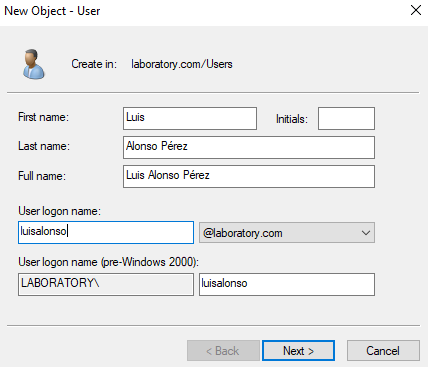
\includegraphics[width=10cm]{DC01/User1.png}
\end{center}
\caption{Usario de dominio.}
\label{DC01-User1}
\end{figure}


\item Usuario de dominio y administrador del dominio (Figura \ref{DC01-User1}). 
\begin{figure}[H] %[ht!] para here [b] para bottom [t] para top
\begin{center}
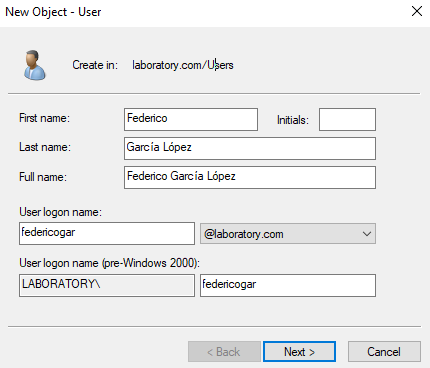
\includegraphics[width=10cm]{DC01/User2.png}
\end{center}
\caption{Usuario de dominio y administrador del dominio.}
\label{DC01-User2}
\end{figure}

Para añadirlo al grupo de administradores de dominio, seleccionamos la opción {\it Add to a group...} (Figura \ref{DC01-User3}).

\begin{figure}[H] %[ht!] para here [b] para bottom [t] para top
\begin{center}
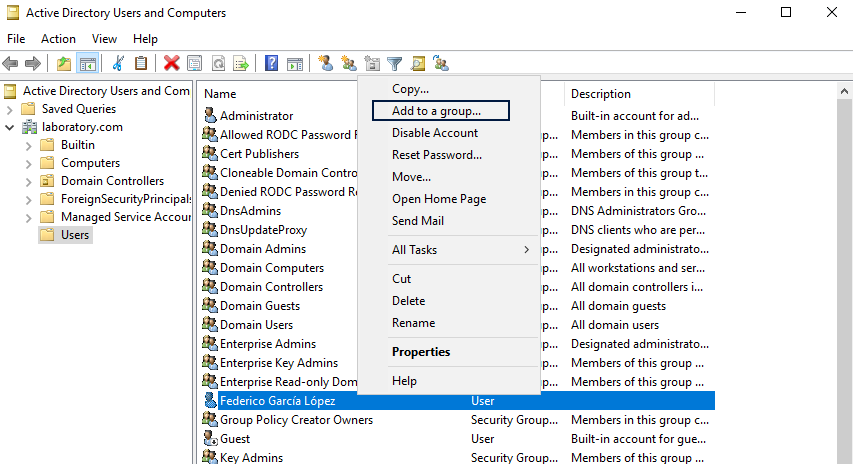
\includegraphics[width=10cm]{DC01/User3.png}
\end{center}
\caption{Añadir el usuario a un grupo.}
\label{DC01-User3}
\end{figure}

Y se añade el grupo {\it Domain Admins} (Figura \ref{DC01-User4}).

\begin{figure}[H] %[ht!] para here [b] para bottom [t] para top
\begin{center}
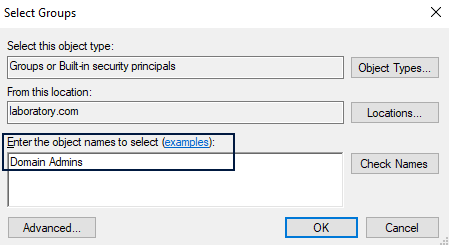
\includegraphics[width=10cm]{DC01/User4.png}
\end{center}
\caption{Grupo Domain Admins.}
\label{DC01-User4}
\end{figure}

\item Usuario de dominio y administrador local en Cliente01 (Figura \ref{DC01-User5}).
\begin{figure}[H] %[ht!] para here [b] para bottom [t] para top
\begin{center}
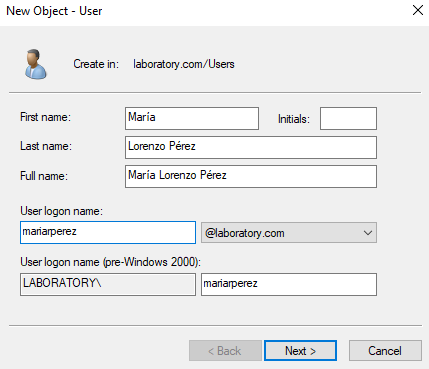
\includegraphics[width=10cm]{DC01/User5.png}
\end{center}
\caption{Usuario de dominio y administrador local.}
\label{DC01-User5}
\end{figure}

Desde una consola con privilegios de administrador local en el Cliente01, ejecutamos el siguiente comando que añade al grupo de administradores el usuario creado previamente. 

\begin{listing}[style=consola, numbers=none]
# net localgroup administrators laboratory\mariarperez /add
\end{listing}

Una vez añadido, es posible loguearse con dicha información (Figura \ref{DC01-User6}).

\begin{figure}[H] %[ht!] para here [b] para bottom [t] para top
\begin{center}
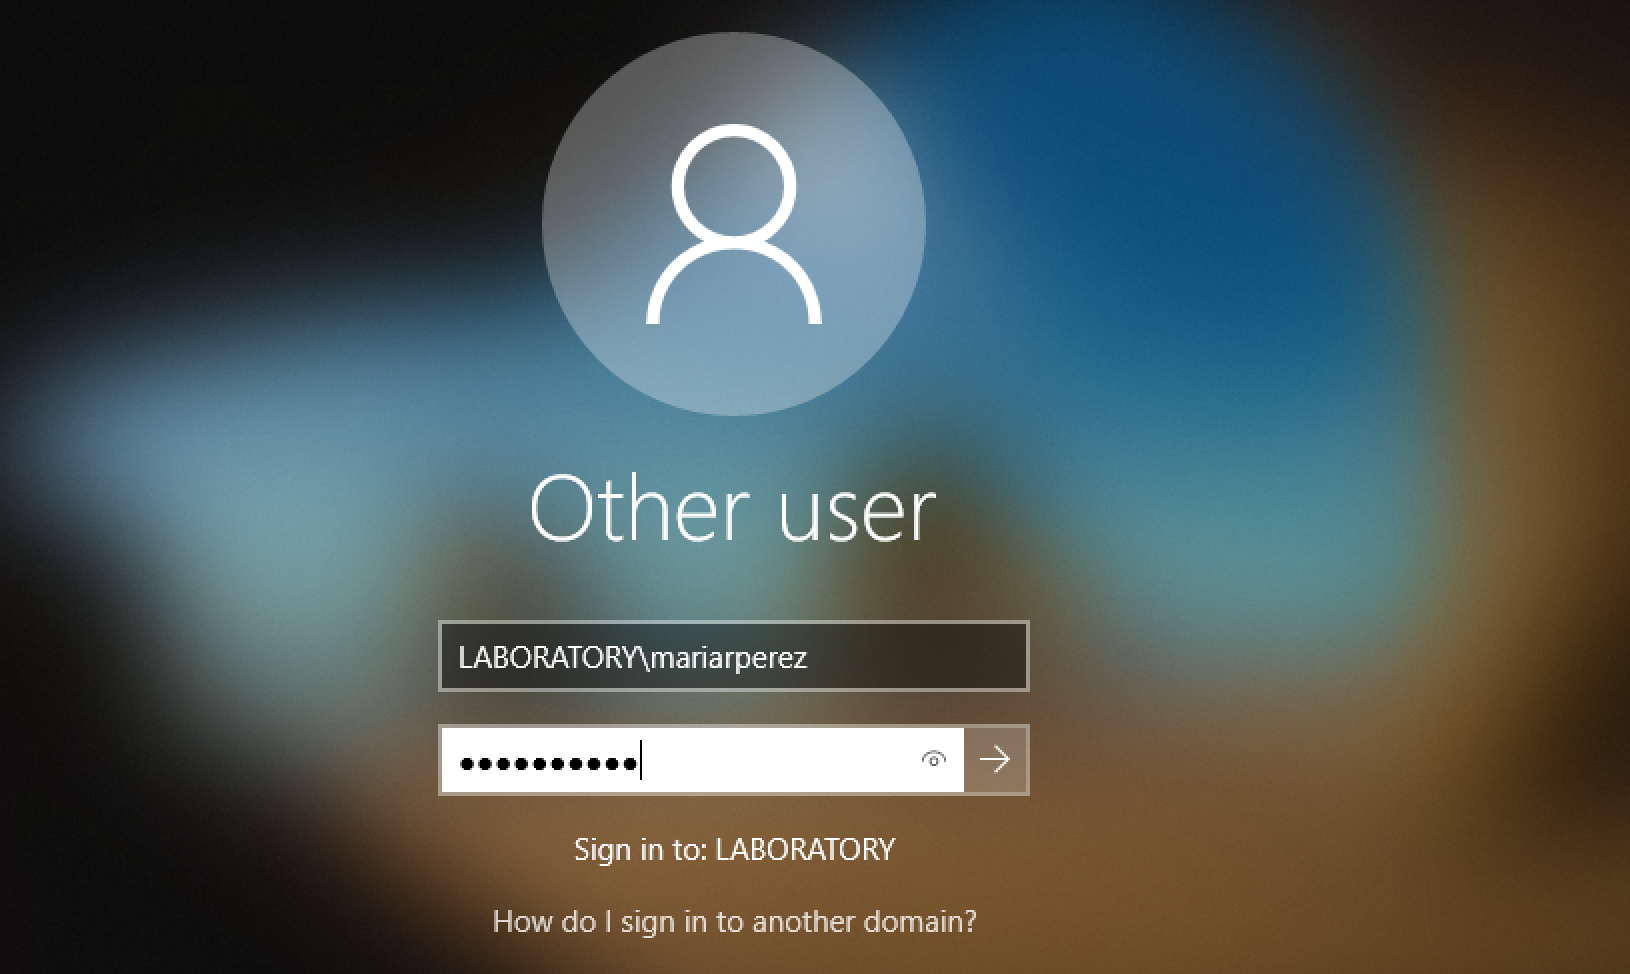
\includegraphics[width=10cm]{DC01/User6.png}
\end{center}
\caption{Inicio de sesión con la cuenta de usuario creada.}
\label{DC01-User6}
\end{figure}


\end{itemize}


